\documentclass[conference]{IEEEtran}
\usepackage{amsmath,amssymb}
\usepackage{graphicx}
\usepackage{cite}
\usepackage{siunitx}
\usepackage{hyperref}

\begin{document}

\title{0.18 µm CMOS における磁性体ラミネートオンチップ\\
マイクロインダクタの提案と LDO ハイブリッド応用}

\author{
  \IEEEauthorblockN{三溝 真一 (Shinichi Samizo)}
  \IEEEauthorblockA{独立研究者 / Project Design Hub}
}

\maketitle

\begin{abstract}
0.18 µm AMS CMOS ノードを対象に、Post-BEOL で磁性体ラミネーションと Patterned Ground Shield (PGS) を付加することで、従来の Air-core スパイラルに内在する低 $Q$・大面積・電流容量不足を克服するオンチップ・マイクロインダクタを提案する。さらに Buck+LDO ハイブリッド電源へ適用し、効率・低ノイズ・高速応答の三立を示す。提案インダクタは 20 MHz 付近で $L=90\text{--}150\,\mathrm{nH},~Q=12\text{--}20,~I_\mathrm{sat}\ge0.5\,\mathrm{A}$ を目標とし、システムとして $\eta_\mathrm{total}\approx 78\text{--}82\%$, Ripple $<1\,\mathrm{mV_{rms}}$, PSRR $>60\,\mathrm{dB}@1\,\mathrm{MHz}$, EMI $-3\sim -6\,\mathrm{dB}$ を示す。成熟ノードに対して +1 工程のみで実装でき、車載・IoT・AMS 混載 IC に即応する。
\end{abstract}

\section{Introduction}
0.18 µm AMS CMOS プロセスは現在も車載・産業・IoT 向け SoC の主力ノードである。%
% (以下 Markdown と同じ内容をセクション分割して移植)

\section{Proposed Method}
Fig.~\ref{fig1} に磁性体ラミネーション・インダクタ断面を示す。

\begin{figure}[htbp]
\centering
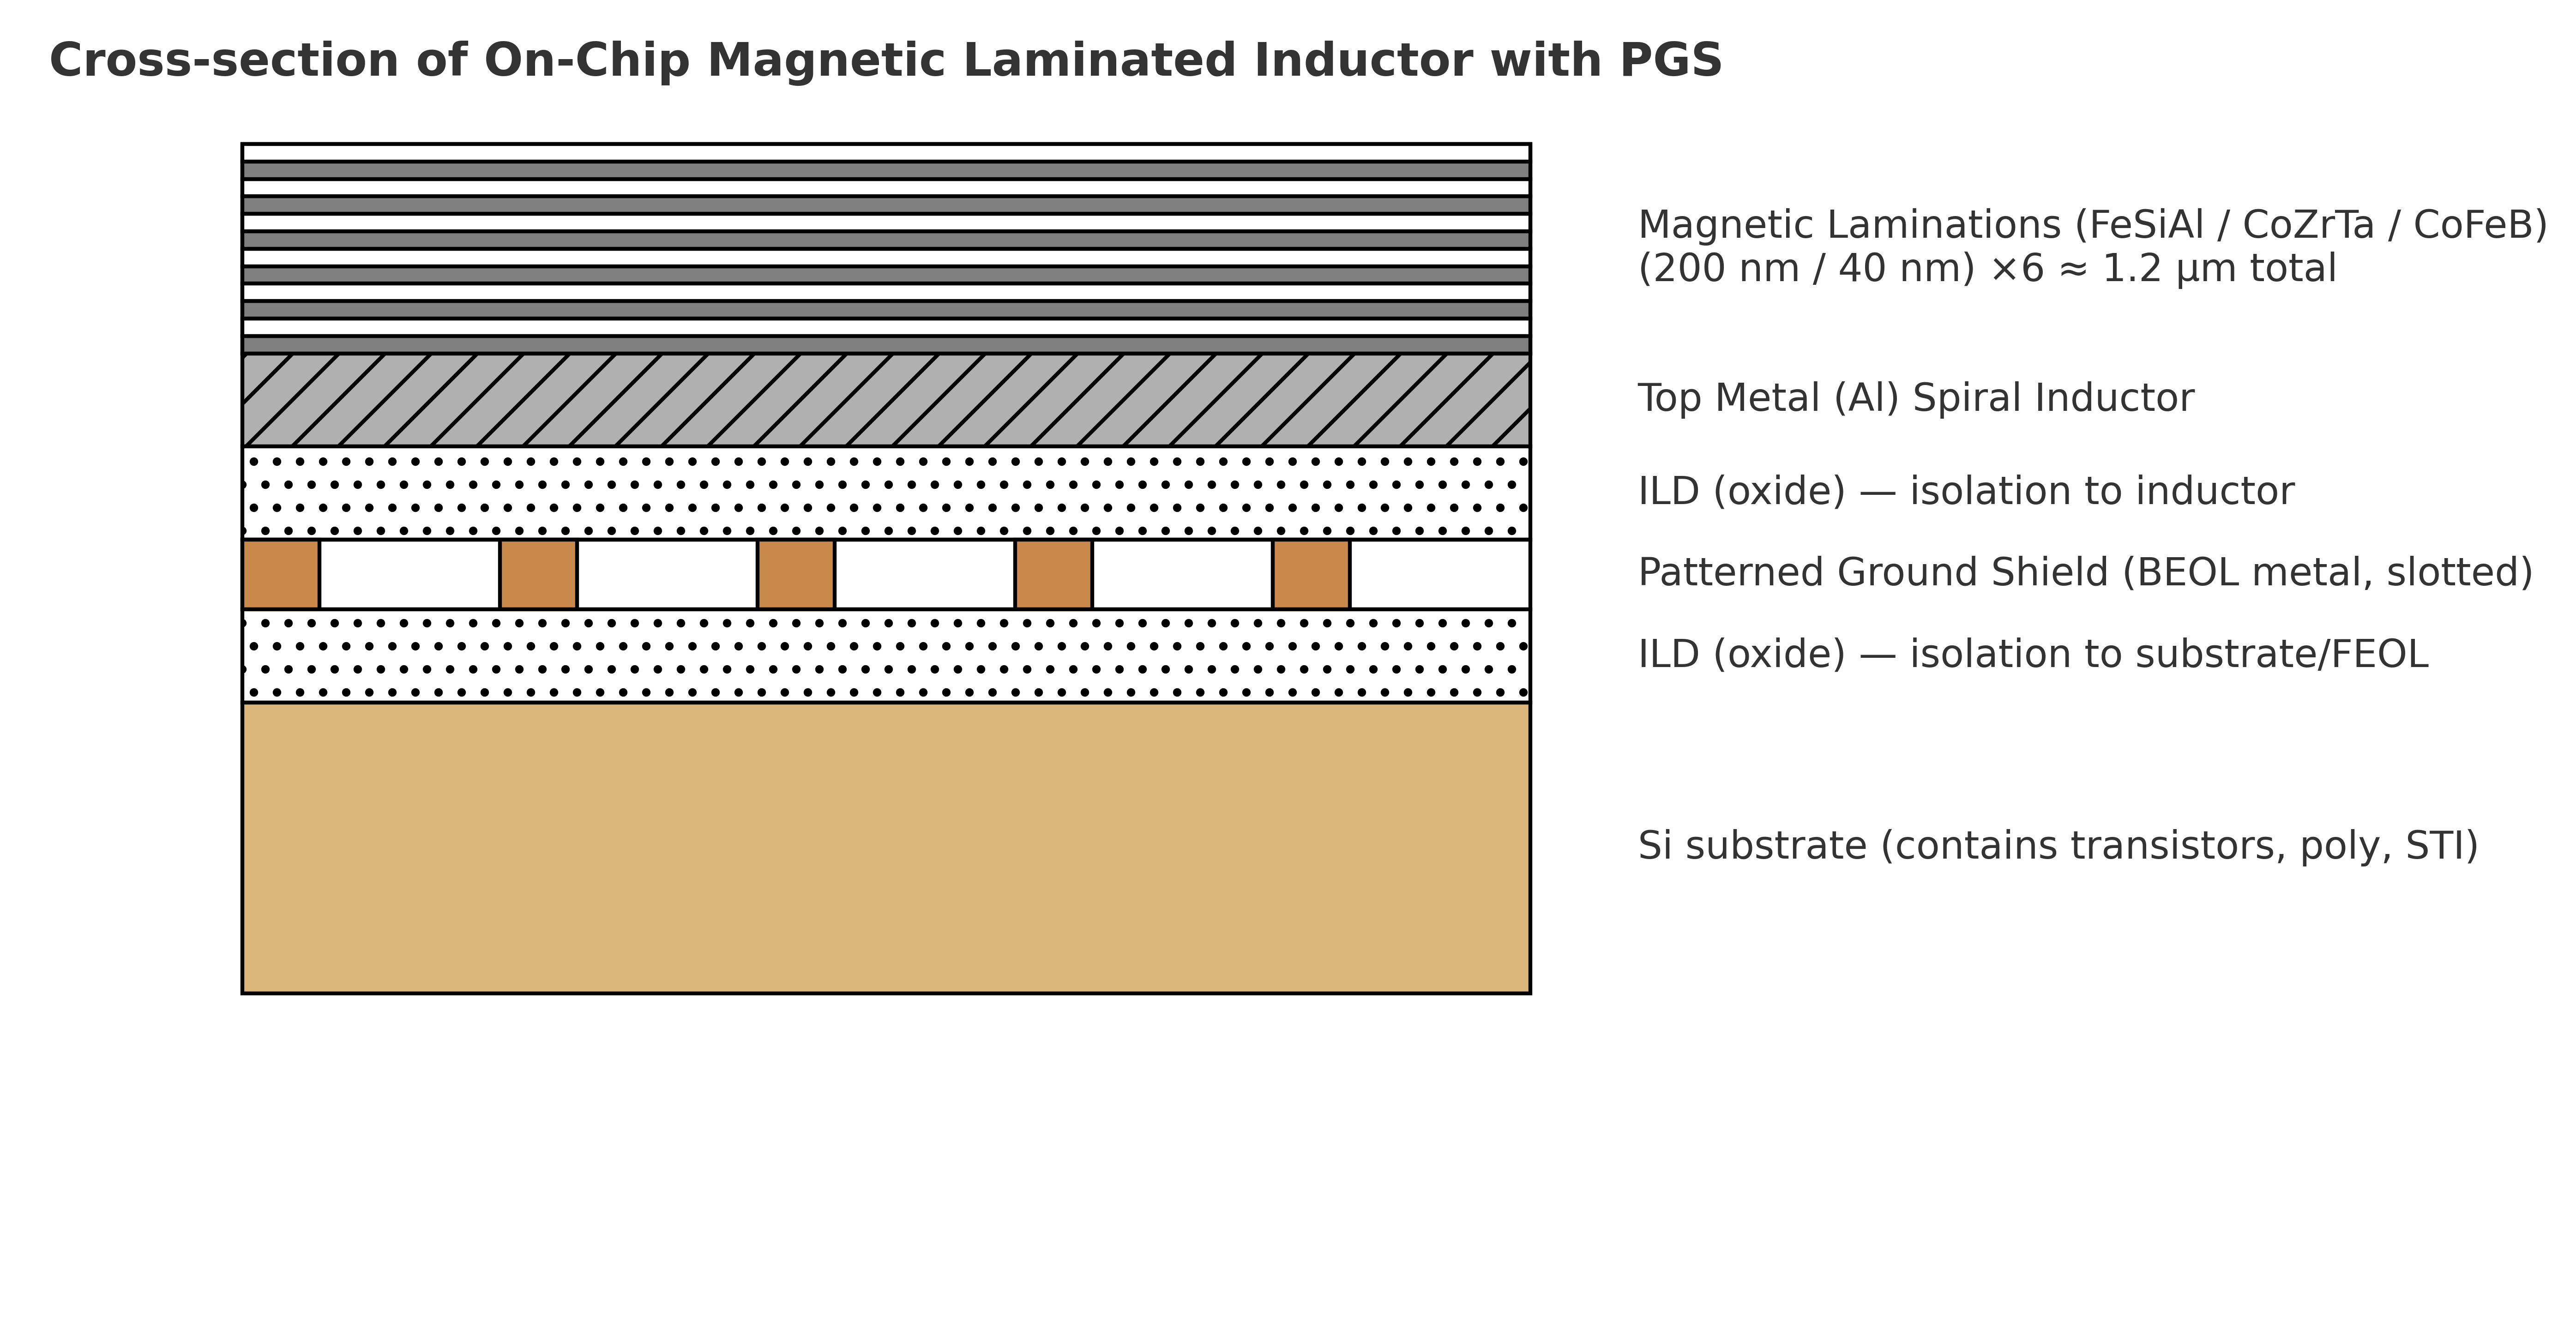
\includegraphics[width=0.8\linewidth]{fig/fig1_laminated_cross_section.png}
\caption{磁性体ラミネーション+PGS の断面概念図}
\label{fig1}
\end{figure}

Fig.~\ref{fig2} に Buck→LDO ハイブリッド電源構成を示す。

\begin{figure}[htbp]
\centering
\includegraphics[width=0.8\linewidth]{fig/fig2_buck_ldo_block.png}
\caption{Buck→LDO ハイブリッド電源構成}
\label{fig2}
\end{figure}

\section{Results}
主要指標の比較を Fig.~\ref{fig3} に示す。

\begin{figure}[htbp]
\centering
\includegraphics[width=0.8\linewidth]{fig/fig3_performance_table.png}
\caption{Air-core と提案手法の主要指標比較(目標)}
\label{fig3}
\end{figure}

PSRR の周波数特性を Fig.~\ref{fig4} に、過渡応答を Fig.~\ref{fig5} に示す。

\begin{figure}[htbp]
\centering
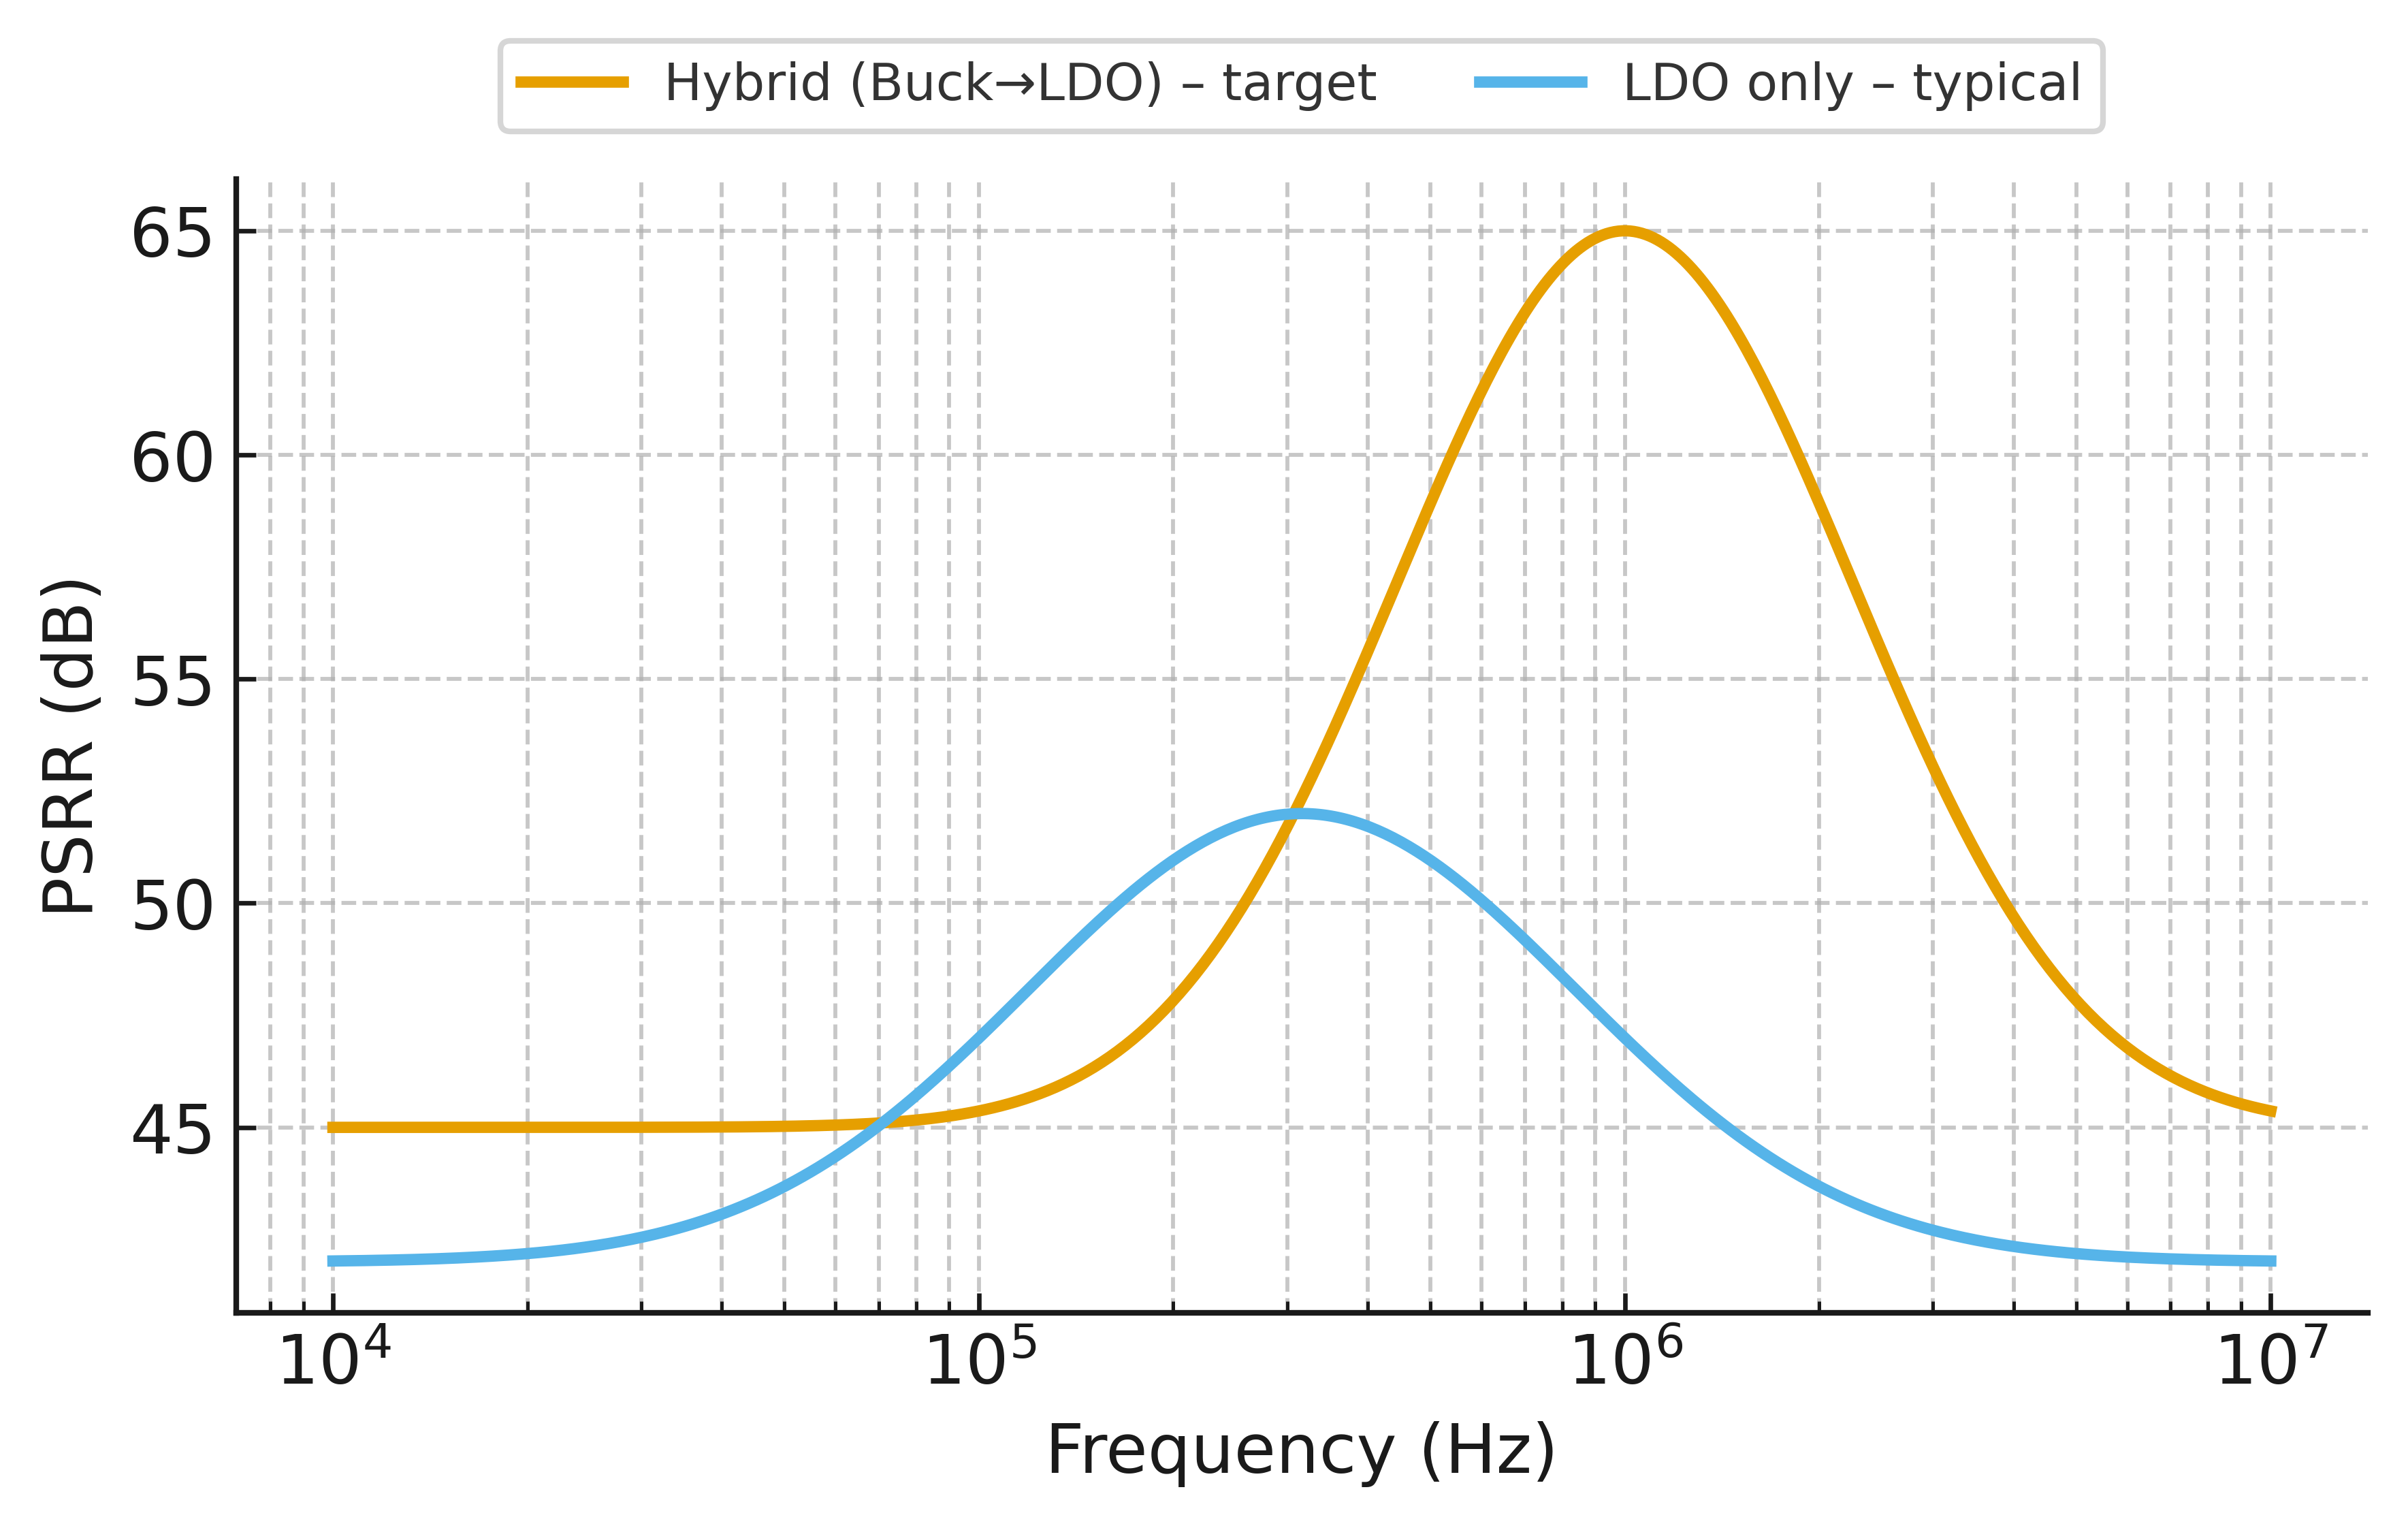
\includegraphics[width=0.8\linewidth]{fig/fig4_psrr_target.png}
\caption{PSRR の周波数特性(目標の概念図)}
\label{fig4}
\end{figure}

\begin{figure}[htbp]
\centering
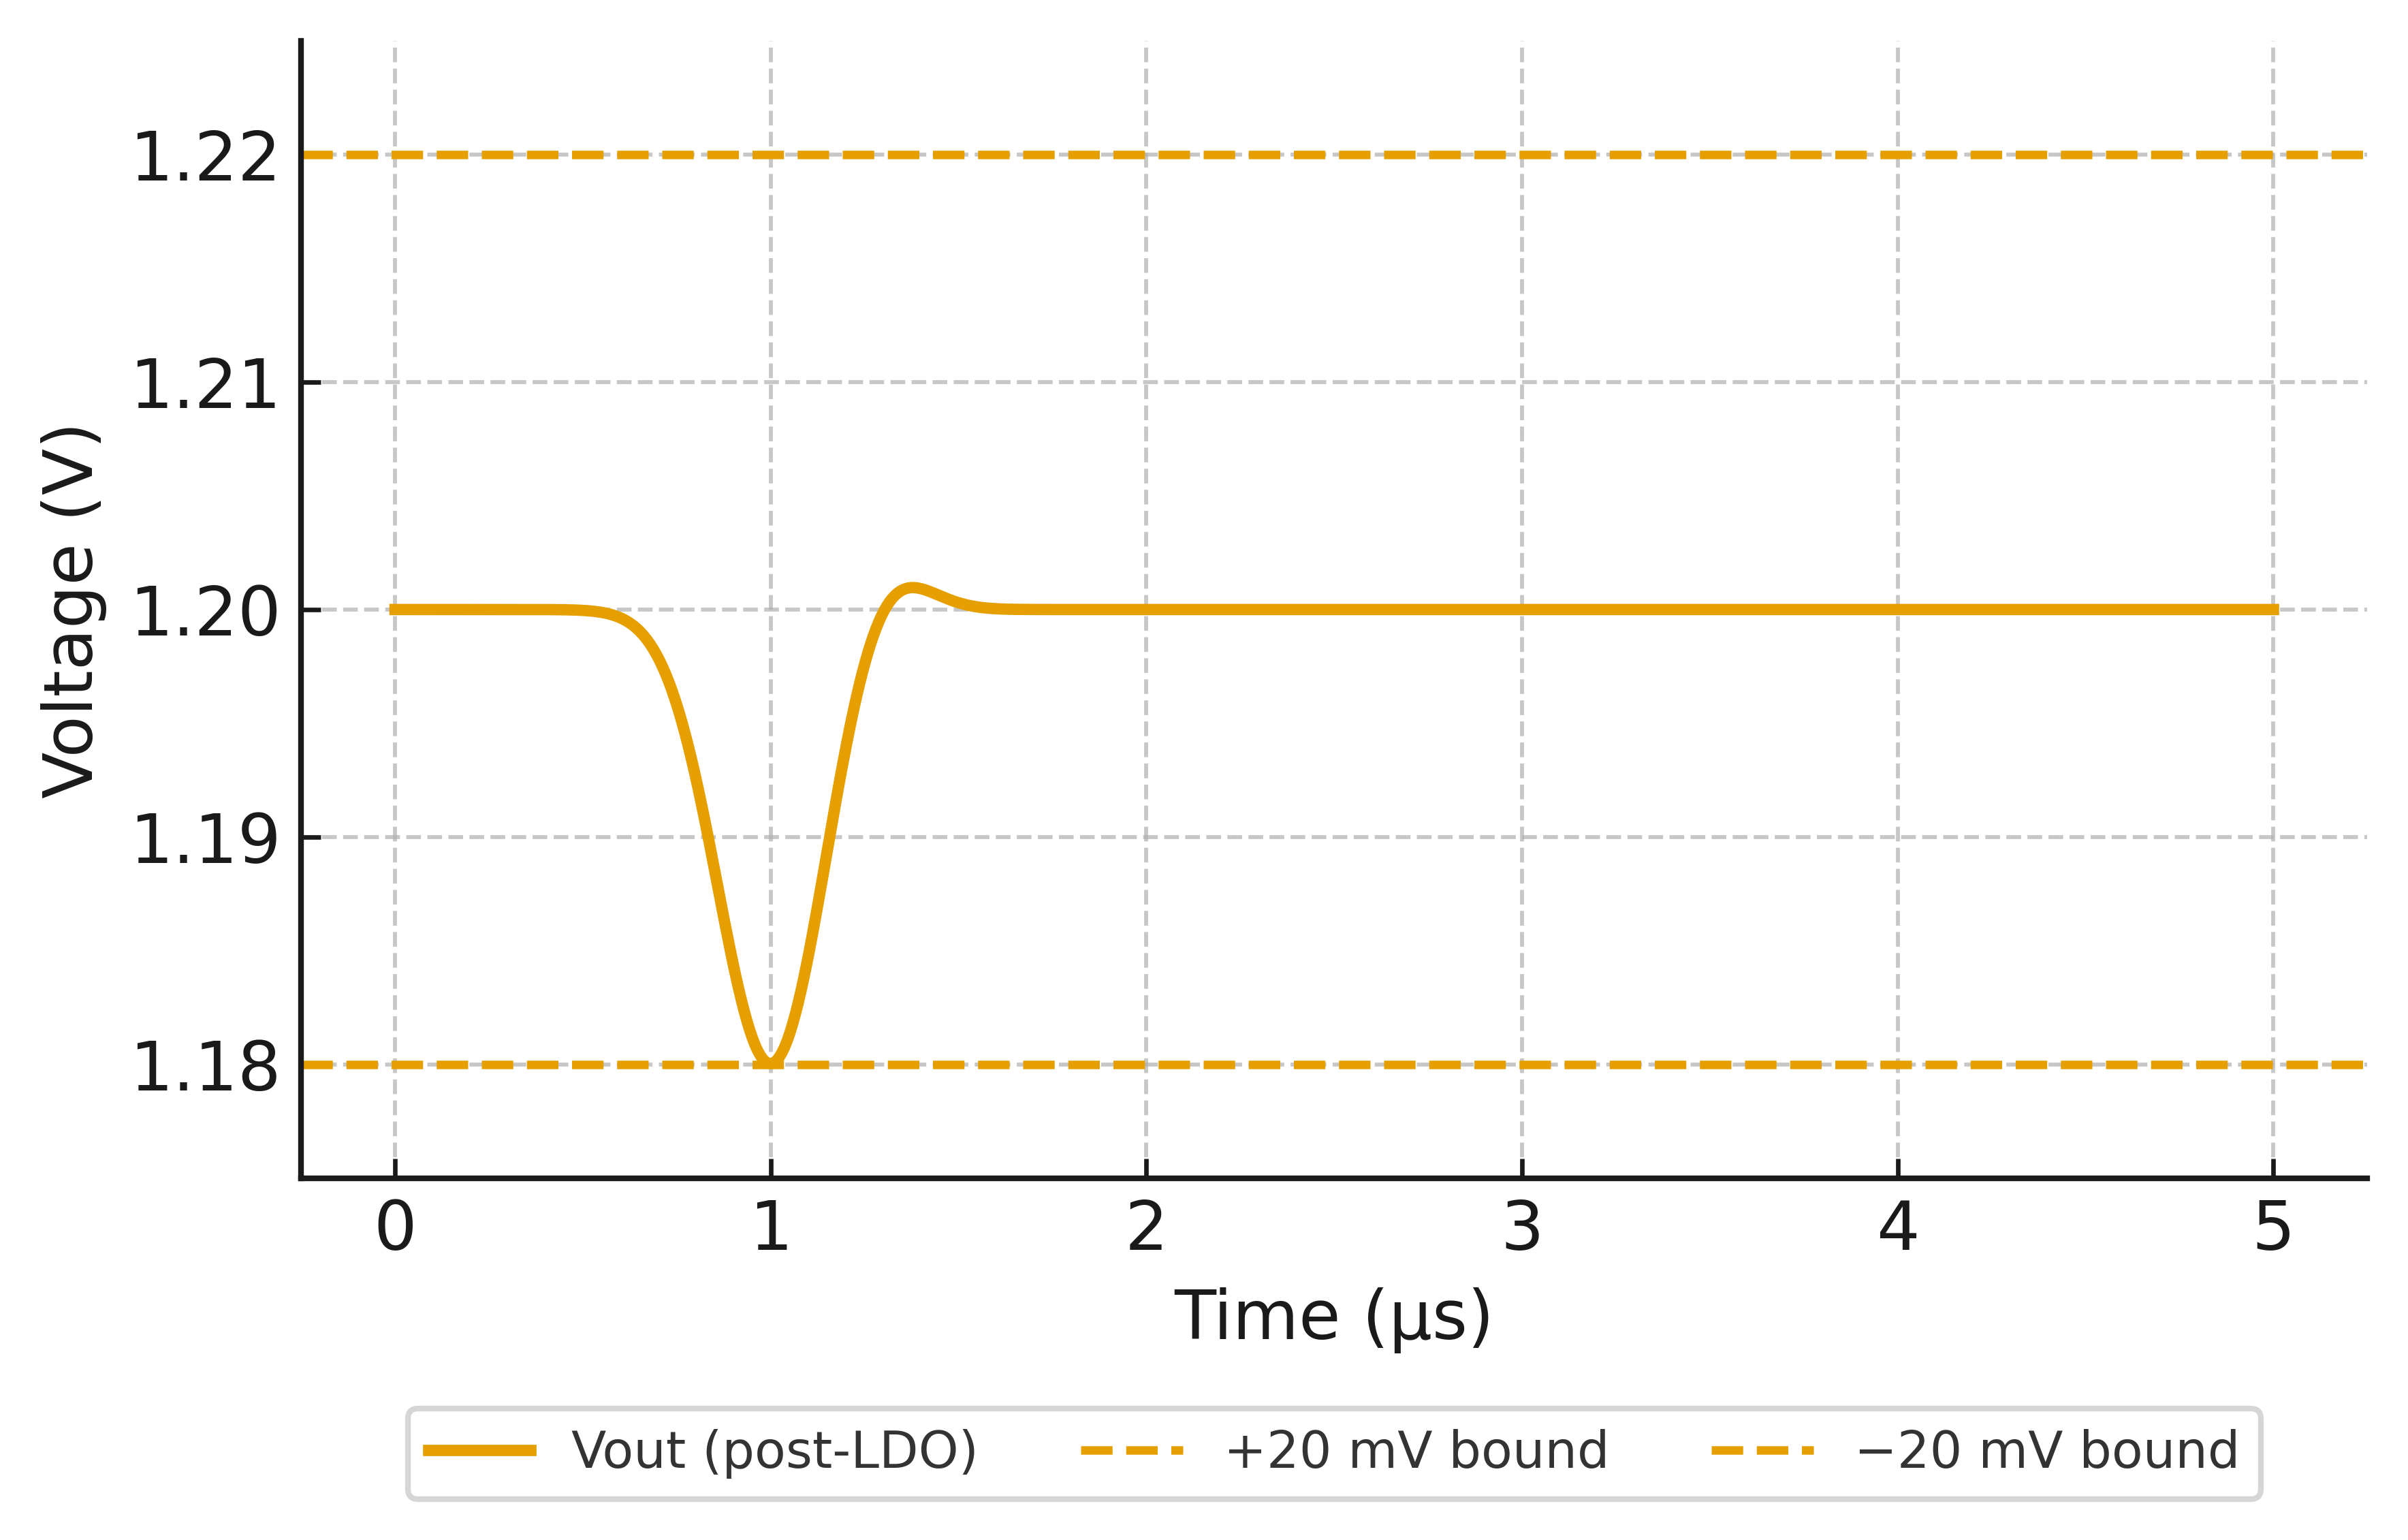
\includegraphics[width=0.8\linewidth]{fig/fig5_transient_response.png}
\caption{0.1 A→0.5 A 過渡応答(±20 mV 以内、概念図)}
\label{fig5}
\end{figure}

\section{Conclusion}
% (Markdown の Conclusion を移植)

\bibliographystyle{IEEEtran}
\begin{thebibliography}{10}
\bibitem{yachi2010} T. Yachi, et al., ``A 20-MHz Fully Integrated Buck Converter with On-Chip Magnetic Inductor in 0.18-µm CMOS,'' \textit{ISSCC}, pp. 300--301, 2010.
\bibitem{park2004} J. Park, et al., ``High-Q Integrated Inductors with Patterned Ground Shields in Standard CMOS Technology,'' \textit{IEEE T-MTT}, vol. 52, no. 2, pp. 471--478, Feb. 2004.
\bibitem{miyake2012} H. Miyake, et al., ``On-Chip Power Supply Noise Reduction Using LDO Regulator Hybrid with Switching Converter,'' \textit{IEEE JSSC}, vol. 47, no. 8, pp. 1928--1937, Aug. 2012.
\bibitem{takamiya2010} M. Takamiya, et al., ``Power Supply Circuits for System-on-Chip,'' \textit{Proc. IEEE}, vol. 98, no. 2, pp. 201--211, Feb. 2010.
\bibitem{makita2013} K. Makita, et al., ``Integrated Magnetic Thin-Film Inductors for On-Chip Power Converters,'' \textit{IEEE T-PEL}, vol. 28, no. 9, pp. 4384--4394, Sept. 2013.
\bibitem{choi2014} S. Choi, et al., ``A 0.18-µm CMOS-Compatible FeSiAl Magnetic Inductor for DC--DC Converters,'' \textit{IEEE EDL}, vol. 35, no. 6, pp. 654--656, June 2014.
\bibitem{kim2015} J. Kim, et al., ``Low-Dropout Regulators for SoC Applications: Design Techniques and Trends,'' \textit{CICC}, pp. 1--8, 2015.
\bibitem{elshazly2020} A. M. Elshazly, et al., ``An Integrated Power Management System for IoT Devices Using Hybrid Buck-LDO Architecture,'' \textit{IEEE TCAS-I}, vol. 67, no. 10, pp. 3348--3360, Oct. 2020.
\bibitem{kawashima2016} Y. Kawashima, et al., ``High-Temperature Reliability of Thin-Film Magnetic Materials for Integrated Inductors,'' \textit{IRPS}, pp. 1--6, 2016.
\bibitem{hu2019} J. Hu, et al., ``Advanced Magnetic Materials for On-Chip Power Inductors: A Review,'' \textit{JMMM}, vol. 491, 165621, 2019.
\end{thebibliography}

\end{document}
